\documentclass[10pt]{beamer}
\usepackage[english]{babel}
\usepackage{graphicx}

\usetheme{Berlin}
\title[Fast Track fit]{Fast Track fit \\ First results with accumulative method}
\author{L. Mirabito}
\institute{IPN Lyon, UCB Lyon, IN2P3, CNRS}
\date{October 29, 2014}

\begin{document}
% \AtBeginSection[]
% {
%   \begin{frame}<beamer>
%     \frametitle{Plan}
%     \tableofcontents[currentsection,currentsubsection]
%   \end{frame}
% }

\setbeamerfont{frametitle}{size=\huge,series=\bfseries}

\begin{frame}
\titlepage
\end{frame}

\section{The method}

\begin{frame}{Accumulation}

\begin{columns}
   \begin{column}{0.5\textwidth}
    \begin{itemize}
    \item Put all stubs in conformal space ($x'=\frac{x}{r^2},y'=\frac{y}{r^2}$)
     \item Calculate all possible combination of 2 layers hits, excluding the inner most one.
     \item Fill an histogram in ($a,b$) space of found combinations
      \item Select bins with $ \ge 3 $ entries (or 4 if more than 150 stubs)
    \end{itemize}
  \end{column}

  \begin{column}{0.65\textwidth}
    \centerline{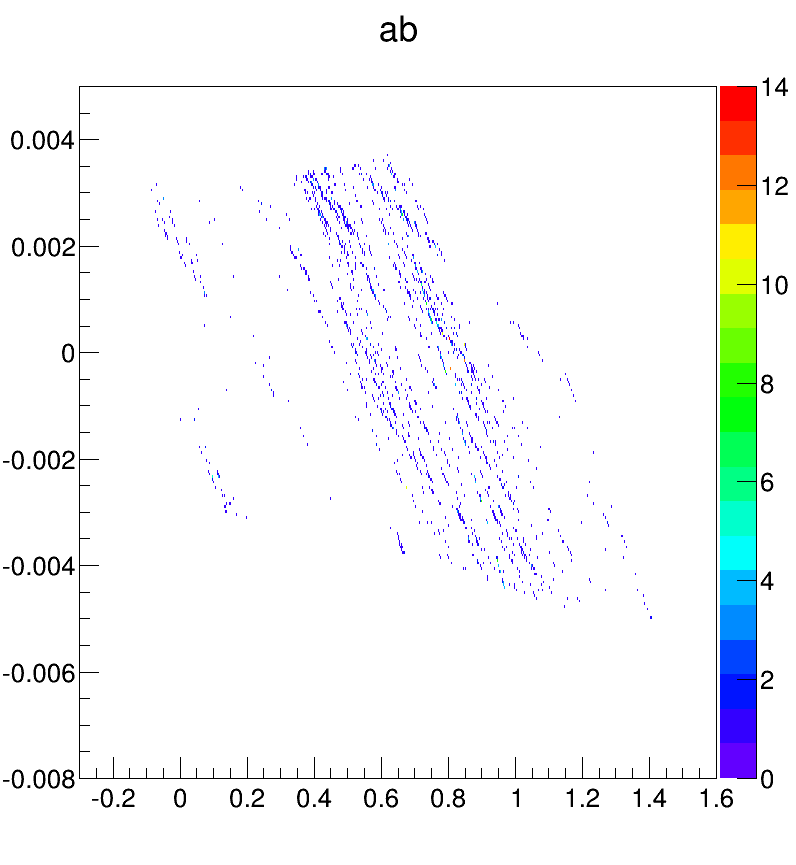
\includegraphics[width=0.9\textwidth]{acumul.png}}
  \end{column}
\end{columns}


\end{frame}
\begin{frame}{Accumulation numbers}
	\centerline{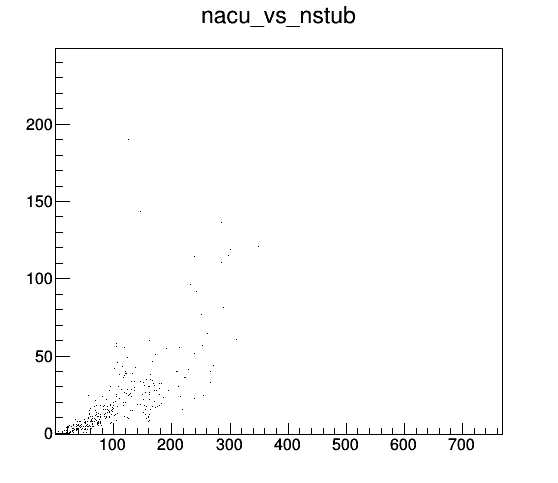
\includegraphics[width=0.9\textwidth,height=0.9\textheight]{nacu_vs_nstub.png}}
\end{frame}
\begin{frame}{Adding hits}

For all candidates
\begin{block}{ Loop on all layers}
  \begin{enumerate}
    \item Skip if layers already touched
    \item Extrapolate the candidate to the layer $ y_{ext} = a_{cand} \times x + b_{cand} $ 
    \item Calculate distance and add nearby hits
  \end{enumerate}
\end{block}
\pause 
\begin{block}{ Fit}
  \begin{itemize}
    \item Requires at least 4 hits in (x,y) and 2 hits in (R,z) selected
    \item Linear regression in the 2 planes
    \item Reject low pt candidates
  \end{itemize}
\end{block}

\end{frame}
\section{Results}


\begin{frame}{Sample \& Results}


\begin{block}{ 140 Pile-up + 4 tops}
  \begin{itemize}
    \item File AMana\_4TPU140\_d01pt2.root
    \item 295 events
    \item 1314 MC tracks with $P_t > 2 GeV$
  \end{itemize}
\end{block}
\pause
\begin{block}	

\begin{tabular}{llllll}
Sector & N Track MC & Ntrack Reco & Efficiency & Fake rate \\
  16   & 1314       & 1736        & 90.64      &  10.05  
\end{tabular}
	
\end{block}
\end{frame}
\begin{frame}{Candidates track statistic}
	\centerline{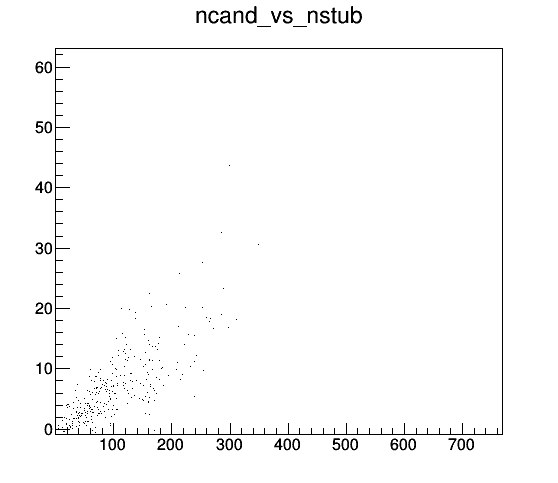
\includegraphics[width=0.9\textwidth,height=0.4\textheight]{ncand_vs_nstub.png}}
	\centerline{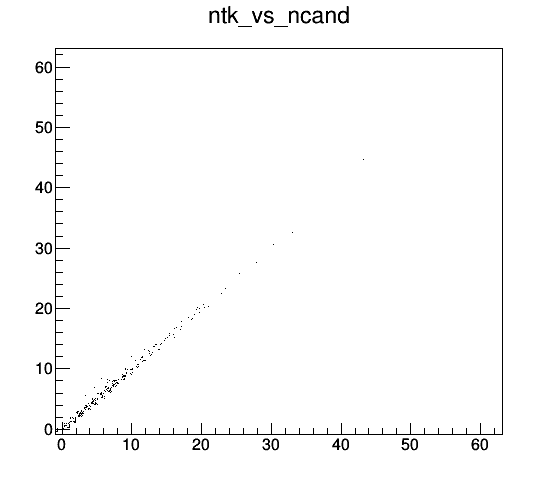
\includegraphics[width=0.9\textwidth,height=0.4\textheight]{ntk_vs_ncand.png}}
\end{frame}

\begin{frame}{Pt resolution}
	\centerline{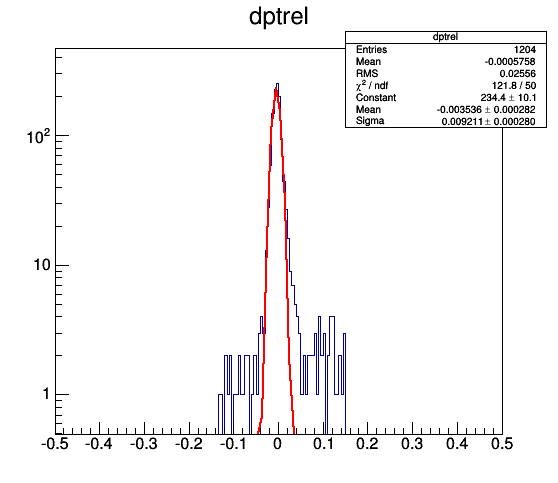
\includegraphics[width=0.9\textwidth,height=0.9\textheight]{dpt_acu.png}}

\end{frame}
\begin{frame}{$\phi$ resolution}
	\centerline{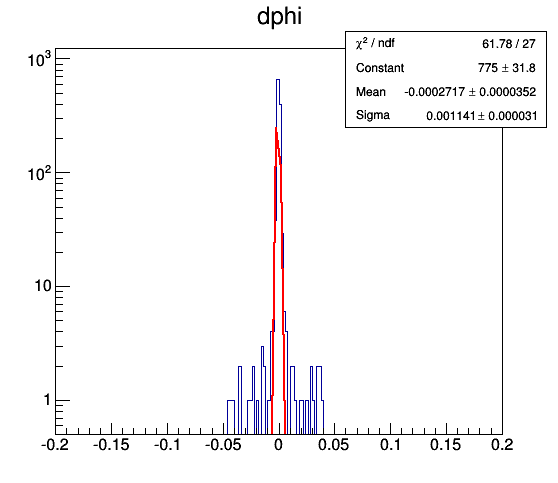
\includegraphics[width=0.9\textwidth,height=0.9\textheight]{dphi_acu.png}}

\end{frame}
\begin{frame}{$\eta$ resolution}
	\centerline{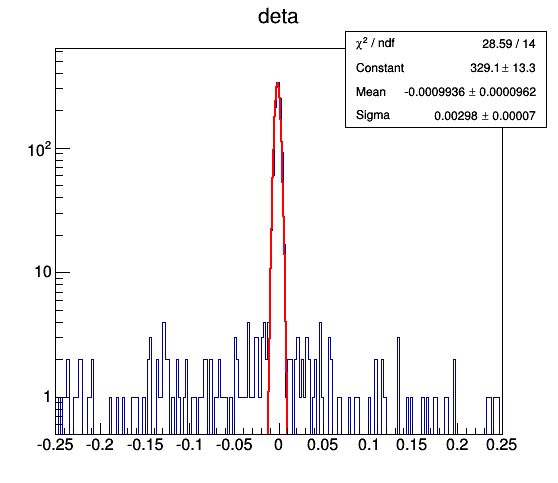
\includegraphics[width=0.9\textwidth,height=0.9\textheight]{deta_acu.png}}

\end{frame}
\begin{frame}{z resolution}
	\centerline{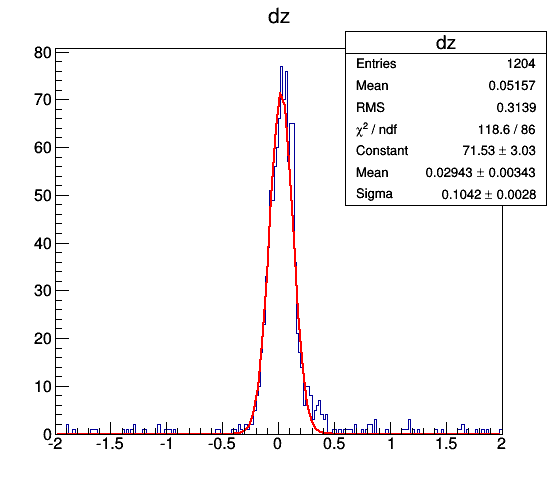
\includegraphics[width=0.9\textwidth,height=0.9\textheight]{dz_acu.png}}

\end{frame}
\section{Conclusion}
\begin{frame}[shrink=2]{Summary}
\begin{block}{Method}
Only the first step is quadratic in stub numbers (without the inner most layer ones ) so the performances should
be comparible to the Hough transform approach.
\par
The final steps are linear in number of stubs and limited ($\le$ 64) in parallel blocks. 

\end{block}
\pause
\begin{block}{First results}
In a barrel sector, high efficiency and relatively low fake rate are achieved. Detail tuning of the algorithm are still to be done and should improve those already good results.
\end{block}
\pause
\begin{block}{Futur}
  \begin{itemize}
    \item Cuts tuning
    \item Sector tuning
    \item GPU \& FPGA implementation
  \end{itemize}
\end{block}
\end{frame}

\end{document}
